\subsection{Algunas aclaraciones sobre las relaciones}

\begin{itemize}
	\item Planteamos la relación 'emitidoPor' entre las clases Alquiler y Empleado de estación para tener en claro quién es el responsable por cada alquiler que se realiza en las distintas estaciones y de esta forma evitar posibles irregularidades en el servicio.
	\item Por el mismo motivo, planteamos las relaciones 'responsabilidad origen' y 'responsabilidad destino' entre las clases Pedido y Empleado de estación. Cuando el sistema emite un pedido de movilización de bicicletas, un empleado de la estación destino se encarga de modificar el stock de dicha estación en base al pedido realizado. Lo mismo sucede en la estación origen.
	\item Planteamos la relación 'emitidoPor' entre las clases Empleado de gobierno e Incorporacion\_bicicletas puesto que queremos evitar posibles errores en la cantidad de bicicletas ingresadas, teniendo así un responsable para cuestionar y sancionar severamente. Al momento de incorporar nuevas bicicletas, el sistema las distribuye según las necesidades actuales de la Red de Ciclovías. 
	\item Consideramos que disponemos de una clase ''today'' con dos atributos: Fecha y Hora, que representan la fecha
	y hora actuales.
	\item Agregamos la clase Orden de Pedido para agregarle un poco de formalidad al proceso de emisión de pedidos.
	\item La relación estaEn - bicicletas entre la clase estación y la clase bicicleta representa el conjunto de 
	bicicletas que actualmente se encuentran en dicha estación (no están siendo alquiladas ni transportadas en
	la fecha y hora actual)
	\item La clase Alquiler modela los alquileres históricos que han sido registrados por el sistema.
	\item La clase Pedido modela los pedidos históricos que han sido registrados por el sistema.
	\item Cada estación registra un conjunto de estadísticas diarias.
\end{itemize}

\begin{figure}[H]
	\centering
	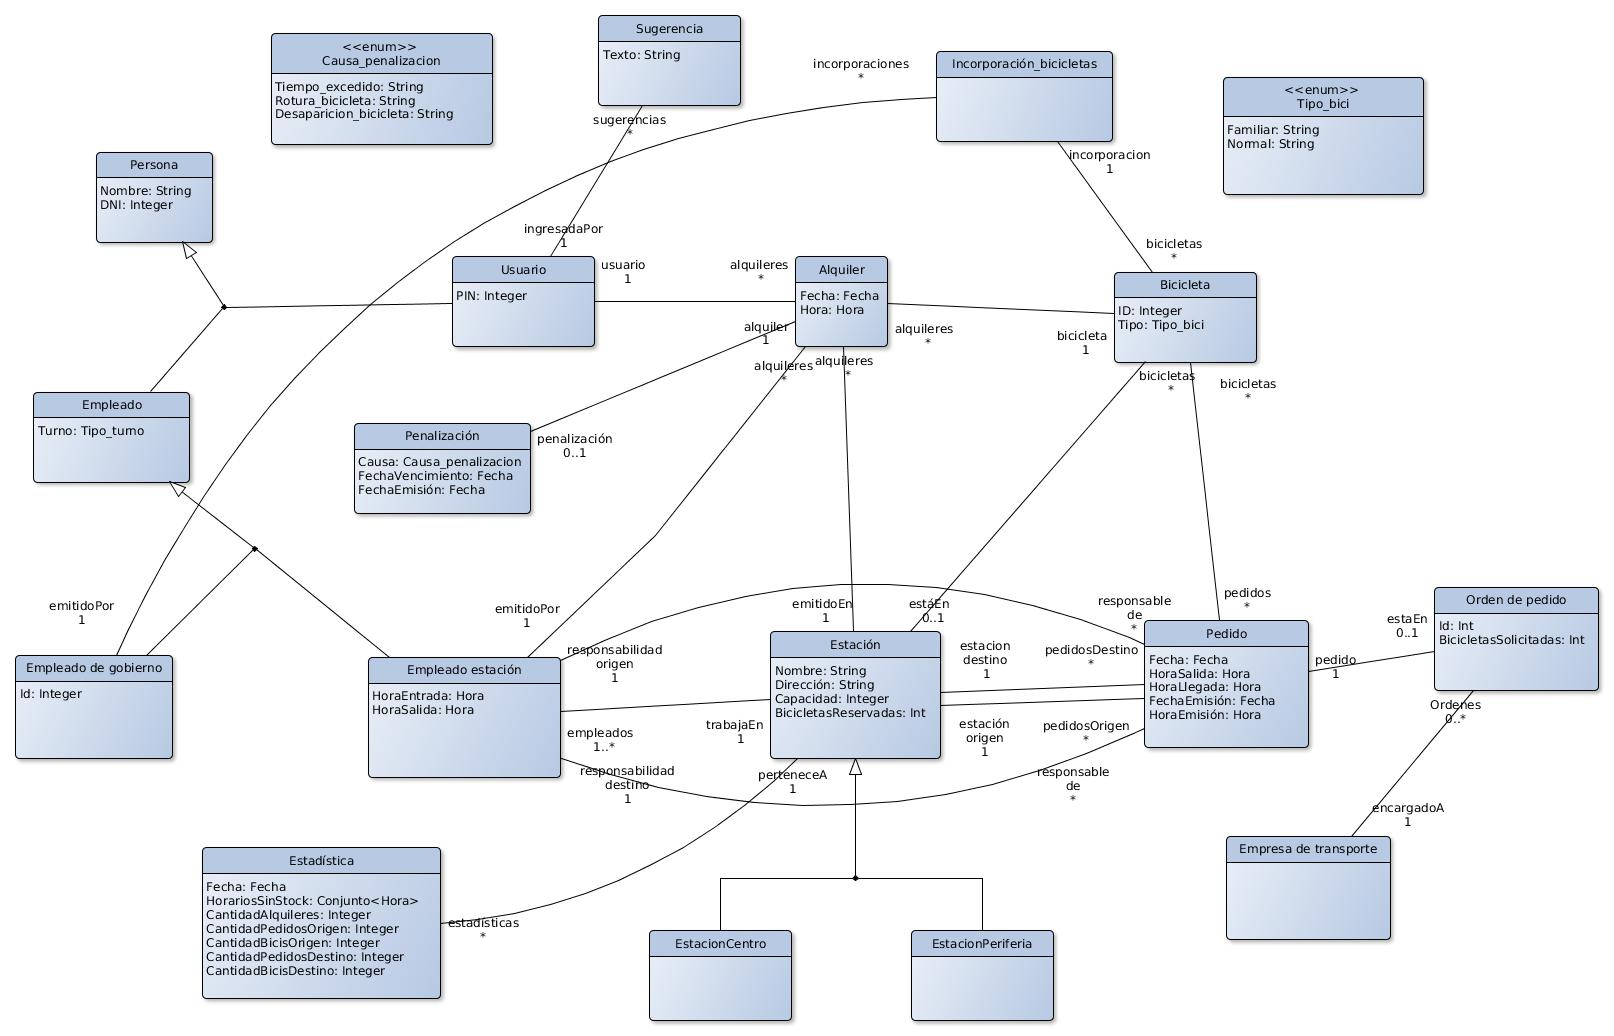
\includegraphics[scale=0.30]{imgs/diagrama_clases.jpg}
	\caption{Diagrama de Clases}
\end{figure}

\subsection{Invariantes en OCL}

\oclInv{Bicicleta}{Pedido.allInstances() $\rightarrow$ forAll(p1 | Pedido.allInstances() $\rightarrow$ forAll(p2 | p1.bicicletas $\rightarrow$ includes(self) $\wedge$ p2.bicicletas $\rightarrow$ includes(self) $\wedge$ p1$\neq$ p2 implies p1.horaSalida $\neq$ p2.horaSalida))}{No hay una bicicleta que esté en dos pedidos distintos para una misma hora}

~

\oclInv{Bicicleta}{(Bicicleta.allInstances() $\rightarrow$ select(b | b.id = self.id) $\rightarrow$ size() ) = 1}{Los identificadores de las bicicletas son distintos}

~

\oclInv{Usuario}{(Usuario.allInstances() $\rightarrow$ select(u | u.DNI = self.DNI) $\rightarrow$ size() ) = 1}{Los DNI's de los usuarios son distintos}

~


%CAMBIAR!!
%\oclInv{Usuario}{(self.penalizacion() $\rightarrow$ size() = 1) implies (
%(self.alquiler $\rightarrow$ size() = 1) implies ((self.alquiler.fecha \ < \ self.penalizacion().fechaEmision $\lor$
%self.alquiler.fecha \ > \ self.penalizacion.fechaVencimiento))))}{Si un usuario está penalizado, no puede alquilar bicicletas entre
%la fecha de origen de la penalización y la fecha de vencimiento}

~

\oclInv{Estacion}{(Estacion.allInstances() $\rightarrow$ select (e| e.nombre = self.nombre) $\rightarrow$ size() ) = 1}
{No hay estaciones con nombres iguales}

~

\oclInv{Estacion}{(Estacion.allInstances $\rightarrow$ select(e | e.direccion = self.direccion) -> size() ) = 1}
{No hay estaciones con direcciones iguales}
	
~

\oclInv{Pedido}{self.estacionOrigen $\neq$ self.estacionDestino}{No hay pedidos con una misma estación como origen y destino}

~

\oclInv{Pedido}{(self.bicicletas $\rightarrow$ size()) < self.estacionOrigen.capacidad}{La estación origen tiene suficiente capacidad como para albergar la cantidad de bicicletas a retirar requerida}

~

\oclInv{Pedido}{(self.bicicletas $\rightarrow$ size()) < self.estacionDestino.capacidad}{La estación destino tiene suficiente
capacidad para albergar la cantidad de bicicletas pedidas}

~

\oclInv{Pedido}{self.Fecha = self.FechaEmisión}{Los pedidos se emiten en la misma fecha en la cual serán transportados}

~

Nota: Para disminuir la cantidad de tiempo en que las bicicletas están reservadas (sin poder ser alquiladas), la hora de 
emisión de los pedidos y la hora en el que se llevan a cabo no pueden estar separadas por más de 5 unidades.
\oclInv{Pedido}{self.HoraSalida - self.HoraEmisión $\leq$ 5}{Los pedidos se emiten en la misma fecha en la cual serán transportados}

~

Nota: Cuando un pedido de \emph{n} bicicletas es emitido, se reservan automáticamente \emph{n} bicicletas en la estación
origen para ser transportadas hacia la estación destino que no podrán ser alquiladas, ya que formarán parte del 
envío.

\oclInv{Pedido}{(today.Fecha() = self.Fecha $\wedge$ today.Hora() $\leq$ self.HoraSalida $\wedge$ self.HoraSalida - today.Hora() <= 5) implies (self.Bicicletas $\rightarrow$ 
forAll (b | b.estaEn $\rightarrow$ size() = 1 $\wedge$ b.estaEn = self.estacionOrigen) )}{Las bicicletas que están en un pedido
no pueden estar alquiladas en el rango de tiempo de 5 horas antes de la hora de salida y deben estar en la estación de origen
del pedido}
%{ ( (self.bicicletas $\rightarrow$ forAll(b | ((b.alquiler $\rightarrow$ size() = 1) implies
%(b.alquiler.Hora $\neq$ self.HoraSalida))))) }

~

\oclInv{Pedido}{(Today.Fecha() = self.Fecha() $\wedge$ self.HoraSalida $\leq$ today.Hora() < self.HoraLlegada) implies (self.bicicletas $\rightarrow$ forAll (b | b.estaEn $\rightarrow$ size() = 0 $\wedge$ b.alquileres $\rightarrow
$ select ( a | a.Fecha = today.Fecha() $\wedge$ a.Hora $\leq$ today.Hora() $\leq$ a.Hora+1) $\rightarrow$ size() = 0))}{Mientras las bicicletas están siendo transportadas no pueden ser alquiladas, y no están en ninguna estación}

~

\oclInv{Pedido}{(today.Fecha() = self.Fecha $\wedge$ today.Hora() = self.HoraLlegada) implies (self.Bicicletas $\rightarrow$ 
forAll (b | b.estaEn $\rightarrow$ size() = 1 $\wedge$ b.estaEn = self.estacionDestino)}{Las bicicletas transportadas
que han llegado recientemente a destino deben estar en la estación destino}

~

\oclInv{EmpleadoEstacion}{(Estacion.allInstances() $\rightarrow$ select ( e | e.id = self.id )) 
$\rightarrow$ size()) = 1 }{No puede haber empleados de estación iguales que trabajen en estaciones distintas}

~

\oclInv{EstacionCentro}{(EstacionPerifera.allInstances()) $\rightarrow$ forAll(e | e.capacidad*2 $\leq$ self.capacidad)}{
Las estaciones del centro tienen más capacidad que las de la periferia. (La proporción del doble parece una aproximación
razonable)}

~

\oclInv{Alquiler}{((self.emitidoEn.empleados $\rightarrow$ select(e | e.id = self.emitidoPor.id)) $\rightarrow$ size()) = 1}{Los alquileres tienen que ser emitidos por algún empleado que trabaje en la estación en donde fue hecho}

~

\oclInv{Pedido}{((self.EstacionDestino.empleados $\rightarrow$ select(e | e.id = self.responsabilidadDestino.id)) $\rightarrow$ size()) = \ 1}{Los pedidos tienen que tener como responsable destino a un empleado que trabaje en la estacion destino}

~


\oclInv{Pedido}{((self.EstacionOrigen.empleados $\rightarrow$ select(e | e.id = self.responsabilidadOrigen.id)) $\rightarrow$ size()) = \ 1}{Los pedidos tienen que tener como responsable origen a un empleado que trabaje en la estacion origen}

%\oclInv{Incorporación\_bicicletas}{(self.bicicletas $\rightarrow$ size()) < \ self.estacionDestino.capacidad}{La estación destino debe tener suficiente capacidad como para albergar la cantidad de bicicletas a incorporar}

~

\oclInv{Alquiler}{(self.Fecha = today.Fecha() $\wedge$ today.Hora() $\leq$ self.Hora + 1)  implies (self.bicicleta.EstaEn $\rightarrow$ size() = 0) }{Si una bicicleta está alquilada entonces no se encuentra en ninguna estación}

~

%%CHEQUEAR

\oclInv{Usuario}{self.alquileres $\rightarrow$ forAll( a | self.alquileres $\rightarrow$ select( p | a.penalizacion $\rightarrow$ size() = 1) $\rightarrow$ forAll(p2 | a.fecha < \ p2.penalizacion.fechaEmision $\lor$ a.fecha > \ p2.penalizacion.fechaVencimiento))}{Ningún usuario puede tener un alquiler cuya fecha coincida con el plazo de alguna penalización}

~

\oclInv{Alquiler}{self.Penalizacion $\rightarrow$ forAll(p | (p.Causa = Desaparicion\_bicicleta) implies (self.bicicleta.estaEn $\rightarrow$ size() = 0 $\wedge$ (self.bicicleta.pedidos $\rightarrow$ forAll (q | not(q.FechaEmision > self.Fecha $\lor$ q.FechaEmision = self.Fecha $\wedge$ q.HoraEmision $\geq$
self.Hora))) $\wedge$ (self.bicileta.alquileres $\rightarrow$ forAll (a | not(a.Fecha > self.Fecha $\lor$ a.Fecha = self.Fecha $\wedge$ a.Hora $\geq$
self.Hora)))) )}{Si una bicicleta desaparece no aparecerá en ningún pedido o alquiler futuro}

~

Nota: $\oplus$ representa el $\lor$ exclusivo (XOR).
\oclInv{Bicicleta}{(self.alquileres $\rightarrow$ exists (a | a.Fecha = today.Fecha() $\wedge$ a.Hora $\leq$ today.Hora() $\leq$
a.Hora()+1)) $\oplus$ (self.estaEn $\rightarrow$ size() = 1) $\oplus$ (self.pedidos.exists ( p | p.fechaEmision = today.Fecha() 
$\wedge$ (p.horaSalida - 5 $\leq$ today.Hora() < p.horaSalida) $\lor$ (p.horaSalida $\leq$ today.Hora() < p.horaLlegada)
)) $\oplus$ (self.alquileres.exists (a | (a.penalizacion $\rightarrow$ size() = 1) $\wedge$ a.penalizacion.Causa\_penalizacion
= Rotura\_bicicleta $\lor$ 

a.penalizacion.Causa\_penalizacion = Desaparicion\_bicicleta))}{Las bicicletas en todo momento están en alguna estación, siendo alquiladas, reservadas en algún
pedido, siendo transportadas o previamente se han roto o han desaparecido}

~

\oclInv{Pedido}{self.responsabilidadOrigen.HoraEntrada $\leq$ self.HoraSalida $\wedge$ self.responsabilidadOrigen.Hora Salida > \ self.HoraSalida}{Los pedidos tienen que tener como responsable origen a un empleado que se encuentre en su puesto de trabajo en el momento en que llega la empresa de transporte}

~

\oclInv{Pedido}{self.responsabilidadDestino.Hora Entrada $\leq$ self.HoraLlegada $\wedge$ self.responsabilidadDestino.Hora Salida > self.HoraLlegada}{Los pedidos tienen que tener como responsable destino a un empleado que se encuentre en su puesto de trabajo en el momento en que llega la empresa de transporte}

~

\oclInv{Usuario}{self.alquileres $\rightarrow$ forAll(a1,a2 | (a1.fecha = a2.fecha) implies (a1.Hora < \ > a2.Hora) )}{Un usuario no puede tener alquileres solapados}

~

\oclInv{Estacion}{self.capacidad $\geq$ self.bicicletas $\rightarrow$ size()}{La cantidad de bicicletas presentes en una estación no supera su capacidad}

~
\oclInv{Estacion}{self.BicicletasReservadas $\leq$ self.bicicletas $\rightarrow$ size()}{La cantidad de bicicletas reservadas en una estación es menor o igual a la cantidad de bicicletas presentes en la misma}

~

\oclInv{Orden de pedido}{self.BicicletasSolicitadas = self.pedido.bicicletas $\rightarrow$ size()}{La cantidad de bicicletas solicitadas en Orden de Pedido coincide con el número de bicicletas solicitadas por el Pedido}

~

\oclInv{Estadística}{self.cantidadAlquileres = self.perteneceA.alquileres $\rightarrow$ select( a | a.Fecha = self.Fecha) $\rightarrow$ size()}{Las estadísticas recolectan correctamente la cantidad de alquileres en una estación en una fecha
determinada}

~

\oclInv{Estadística}{self.cantidadPedidosOrigen = self.perteneceA.pedidosOrigen $\rightarrow$ select( p | p.Fecha = self.Fecha) $\rightarrow$ size()}{Las estadísticas recolectan correctamente la cantidad de pedidos en los cuales se retiran bicicletas de la estación en una fecha determinada}

~

\oclInv{Estadística}{self.cantidadPedidosDestino = self.perteneceA.pedidosDestino $\rightarrow$ select( p | p.Fecha = self.Fecha) $\rightarrow$ size()}{Las estadísticas recolectan correctamente la cantidad de pedidos en los cuales ingresan bicicletas a la estación en una fecha determinada}

~

\oclInv{Estadística}{self.cantidadBicisOrigen = self.perteneceA.pedidosOrigen $\rightarrow$ select( p | p.Fecha = self.Fecha) $\rightarrow$ collect( b | b.biciletas $\rightarrow$ size() ) $\rightarrow$ sum()}{Las estadísticas recolectan correctamente la cantidad de bicicletas que se retiran de la estación para un pedido en una fecha determinada}

~

\oclInv{Estadística}{self.cantidadBicisDestino = self.perteneceA.pedidosDestino $\rightarrow$ select( p | p.Fecha = self.Fecha) $\rightarrow$ collect( b | b.biciletas $\rightarrow$ size() ) $\rightarrow$ sum()}{Las estadísticas recolectan correctamente la cantidad de bicicletas que ingresan en una estación para un pedido en una fecha determinada}

~

\oclInv{Pedido}{(self.Fecha = today.Fecha() $\wedge$ self.horaSalida $\leq$ today.Hora() $\wedge$ today.Hora() $\leq$ self.horaLlegada) implies (self.estacionOrigen.bicicletas $\rightarrow$ size() $\geq$ self.bicicletas $\rightarrow$ size() )}{La cantidad de bicicletas solicitadas en un pedido no supera al stock de la estación origen}

~

\oclInv{Pedido}{(self.Fecha = today.Fecha() $\wedge$ self.horaSalida $\leq$ today.Hora() $\wedge$ today.Hora() $\leq$ self.horaLlegada) implies (self.estacionDestino.Capacidad - self.estacionDestino.bicicletas $\rightarrow$ size() $\geq$ self.bicicletas $\rightarrow$ size() )}{La cantidad de bicicletas solicitadas en un pedido no supera la capacidad de la estación destino}

%Otras para agregar:
%\begin{itemize}
%\item No puede haber una bicicleta alquilada que este en una estacion (listo)
%\item No se puede superar la capacidad de la estacion al incorporar nuevas bicicletas. (listo)
%\item El pedido tiene que tener como responsable a un empleado que trabaje en la estacion destino. (listo)
%\item El alquiler tiene que ser emitido por un empleado que trabaje en la estación en donde fue hecho. (listo)
%\item No se solapan alquileres y penalizaciones. (listo)
%\item Hay una penalizacion si y solo si hay un alquiler indebido.
%\item La capacidad nunca es superada por la cantidad de bicicletas presentes (listo)
%\end{itemize}





